\documentclass[a4paper]{report}
\usepackage{graphicx}
\usepackage{xspace,ifthen,epsfig}
\usepackage{cite}
\usepackage{color}
\usepackage{fancybox}
\usepackage{float}
\usepackage{subfigure}
\usepackage{longtable} 
\usepackage{tabularx} 
\usepackage{ltxtable} 
\usepackage{times}
\usepackage[table]{xcolor}
\usepackage{url}
\usepackage{listings}
\usepackage{amsmath}
\usepackage{dsfont}
\usepackage[american]{babel}
\usepackage[utf8]{inputenc}
\usepackage{fancyhdr}
\usepackage{booktabs}
\usepackage{tikz,pgfplots}
\usepackage{todonotes}
\usepackage{footmisc}
\usepackage{marvosym}
\usepackage{hyperref}

\usetikzlibrary{pgfplots.statistics}
\pgfplotsset{
  width=80mm,height=60mm,
  major grid style={thin,dotted,color=black!50},
  minor grid style={thin,dotted,color=black!50},
  grid,
  every axis/.append style={
    line width=0.5pt,
    tick style={
      line cap=round,
      thin,
      major tick length=4pt,
      minor tick length=2pt,
    },
  },
  /pgf/number format/1000 sep={},
  legend cell align=left,
  legend pos=north west,
  log y ticks with fixed point/.style={
      yticklabel={
        \pgfkeys{/pgf/fpu=true}
        \pgfmathparse{exp(\tick)}%
        \pgfmathprintnumber[fixed relative, precision=3]{\pgfmathresult}
        \pgfkeys{/pgf/fpu=false}
      }
  },
}

\begin{document}


\begin{figure}[H]
    \centering
    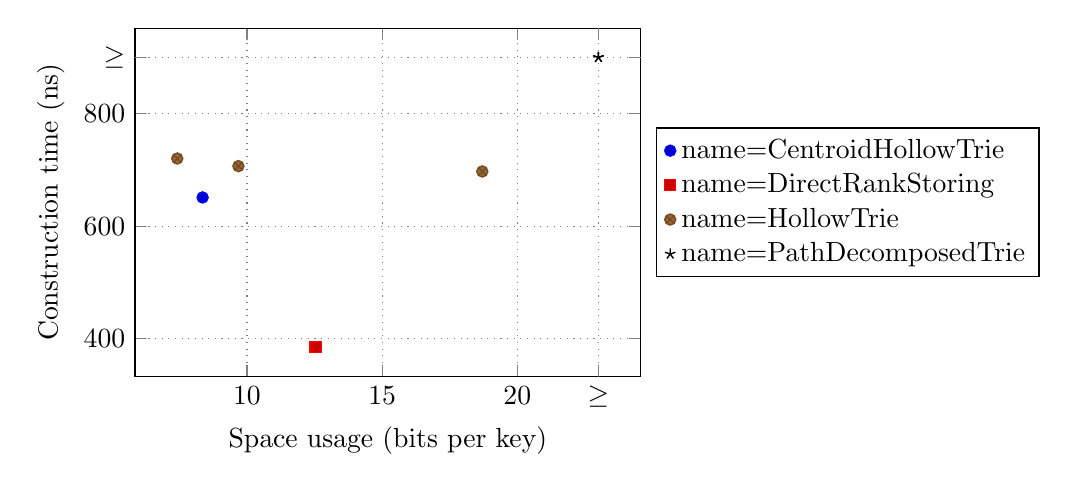
\begin{tikzpicture}
        \begin{axis}[
            title={},
            xlabel={Space usage (bits per key)},
            ylabel={Construction time (ns)},
            legend style={at={(1.03,0.5)},anchor=west},
            legend columns=1,
            only marks,
            extra x ticks={23},
            extra x tick labels={$\geq$},
            extra y ticks={900},
            extra y tick labels={$\geq$},
          ]
          % IMPORT-DATA urls data/uk-2007-05.urls.txt
          %% MULTIPLOT(name)
          %%   SELECT
          %%     MIN(bitsPerElement, 23) as x,
          %%     MIN(1000000.0*constructionTimeMilliseconds/N, 900) as y,
          %%     name
          %%   FROM urls
          %%   ORDER BY name,x
          \addplot coordinates { (8.35901,651.05) };
          \addlegendentry{name=CentroidHollowTrie};
          \addplot coordinates { (12.5432,384.838) };
          \addlegendentry{name=DirectRankStoring};
          \addplot coordinates { (7.42151,720.241) (9.68466,706.737) (18.7052,697.228) };
          \addlegendentry{name=HollowTrie};
          \addplot coordinates { (23,900) (23,900) };
          \addlegendentry{name=PathDecomposedTrie};
        \end{axis}
    \end{tikzpicture}
    \caption{Space usage versus construction time of different competitors on the \texttt{uk-2007-05.urls} data set. Bottom left corner is better.}
\end{figure}

\end{document}
